\documentclass[12pt, a4paper]{article}
\usepackage{ctex}
\usepackage{amsmath}
\usepackage{amsfonts}
\usepackage{latexsym}
\usepackage[margin=1in]{geometry}
\usepackage{color}
\definecolor{bgGray}{RGB}{36, 36, 36}
\usepackage{supertabular}
\usepackage{fontspec}
\newfontfamily\courier{Courier}
\usepackage{xcolor}
\usepackage{tikz}
\title{Testcase 3 Tikz Graphics}
\author{OOP2}
\begin{document}
\maketitle

\tableofcontents

\newpage

\section{Graph1}

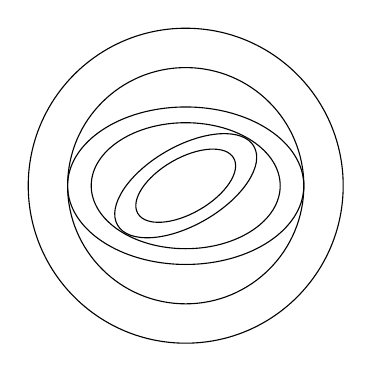
\begin{tikzpicture}
\draw

(0,0) circle [radius=1.5];
\draw

(0,0) circle (2cm);
\draw

(0,0) circle [x radius=1.5cm, y radius=10mm];
\draw

(0,0) circle (1.2cm and 8mm);
\draw

(0,0) circle [x radius=1cm, y radius=5mm, rotate=30];
\draw

[rotate=30] (0,0) ellipse (20pt and 10pt);
\end{tikzpicture}

\section{Graph2}

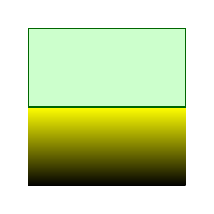
\begin{tikzpicture}
\draw

(0,0) rectangle (1,1);
\shade

[top color=yellow, bottom color=black] (0,0) rectangle (2,-1);
\filldraw

[fill=green!20!white, draw=green!40!black] (0,0) rectangle (2,1);
\end{tikzpicture}

\section{Graph3}

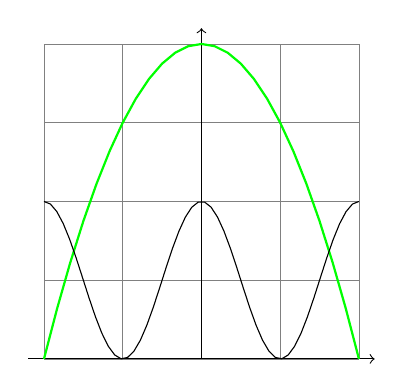
\begin{tikzpicture}
\draw

[help lines] (-2,0) grid (2,4);
\draw

[->] (-2.2,0) -- (2.2,0);
\draw

[->] (0,0) -- (0,4.2);
\draw

[green, thick, domain=-2:2] plot (\x, {4-\x*\x});
\draw

[domain=-2:2, samples=50] plot (\x, {1+cos(pi*\x r)});
\end{tikzpicture}

\end{document}
